\documentclass[11pt]{scrartcl}
\usepackage[T1]{fontenc}
\usepackage[a4paper, left=3cm, right=2cm, top=2cm, bottom=2cm]{geometry}
\usepackage[activate]{pdfcprot}
\usepackage[ngerman]{babel}
\usepackage[parfill]{parskip}
\usepackage[utf8]{inputenc}
\usepackage{kurier}
\usepackage{amsmath}
\usepackage{amssymb}
\usepackage{xcolor}
\usepackage{epstopdf}
\usepackage{txfonts}
\usepackage{fancyhdr}
\usepackage{graphicx}
\usepackage{prettyref}
\usepackage{hyperref}
\usepackage{eurosym}
\usepackage{setspace}
\usepackage{units}
\usepackage{eso-pic,graphicx}
\usepackage{icomma}
\usepackage{pdfpages}

\definecolor{darkblue}{rgb}{0,0,.5}
\hypersetup{pdftex=true, colorlinks=true, breaklinks=false, linkcolor=black, menucolor=black, pagecolor=black, urlcolor=darkblue}



\setlength{\columnsep}{2cm}


\newcommand{\arcsinh}{\mathrm{arcsinh}}
\newcommand{\asinh}{\mathrm{arcsinh}}
\newcommand{\ergebnis}{\textcolor{red}{\mathrm{Ergebnis}}}
\newcommand{\fehlt}{\textcolor{red}{Hier fehlen noch Inhalte.}}
\newcommand{\betanotice}{\textcolor{red}{Diese Aufgaben sind noch nicht in der Übung kontrolliert worden. Es sind lediglich meine Überlegungen und Lösungsansätze zu den Aufgaben. Es können Fehler enthalten sein!!! Das Dokument wird fortwährend aktualisiert und erst wenn das \textcolor{black}{beta} aus dem Dateinamen verschwindet ist es endgültig.}}
\newcommand{\half}{\frac{1}{2}}
\renewcommand{\d}{\, \mathrm d}
\newcommand{\punkte}{\textcolor{white}{xxxxx}}
\newcommand{\p}{\, \partial}
\newcommand{\dd}[1]{\item[#1] \hfill \\}

\renewcommand{\familydefault}{\sfdefault}
\renewcommand\thesection{}
\renewcommand\thesubsection{}
\renewcommand\thesubsubsection{}


\newcommand{\themodul}{Halbleiter und Nanostrukturen - Fragen zum Bipolartransistor}
\newcommand{\thetutor}{Prof. Förster}
\newcommand{\theuebung}{Praktikum}

\pagestyle{fancy}
\fancyhead[L]{\footnotesize{C. Hansen}}
\chead{\thepage}
\rhead{}
\lfoot{}
\cfoot{}
\rfoot{}

\title{\themodul{}, \theuebung{}, \thetutor}


\author{Christoph Hansen \\ {\small \href{mailto:chris@university-material.de}{chris@university-material.de}} }

\date{}


\begin{document}

\maketitle

Dieser Text ist unter dieser \href{http://creativecommons.org/licenses/by-nc-sa/4.0/}{Creative Commons} Lizenz veröffentlicht.

\textcolor{red}{Ich erhebe keinen Anspruch auf Vollständigkeit oder Richtigkeit. Falls ihr Fehler findet oder etwas fehlt, dann meldet euch bitte über den Emailkontakt.}

\tableofcontents


\newpage

\section{Frage 1}

Halbleiter sind Leiter, bei denen die elektrische Leitfähigkeit von der Temperatur abhängt. Man unterschiedet dabei grob zwischen Heiß- und Kaltleitern. Zudem gibt es Elementhalbleiter, diese bestehen nur aus einem Elemnt und Verbindungshalbleitern.


\section{Frage 2}

Wenn ein Halbleiter dotiert ist, dann wurde das Halbleitermaterial zusätzlich noch mit einem Element, das mehr Elektronen als das Halbleitermaterial hat (n-Dotierung) oder mit einem Element, das weniger Elektronen als das Halbleitermaterial hat (p-Dotierung) versetzt.

\section{Frage 3}

Die Energie zum Überwinden der Diffusionsspannung kann in Form elektrischer Energie zugeführt werden. Diese Energie vergrößert entweder den Potentialwall oder verkleinert ihn.

Durch Anlegen einer äußeren Spannung in Sperrrichtung (+ am n-Kristall, - am p-Kristall) wird das elektrische Feld der Sperrschicht verstärkt und die Ausdehnung der Raumladungszone vergrößert. Elektronen und Löcher werden von der Sperrschicht weggezogen. Es fließt nur ein sehr geringer Strom, erzeugt durch Minoritätsladungsträger (Sperrstrom), außer die Durchbruchspannung wird überschritten.

Bei Polung in Durchlassrichtung (+ am p-Kristall, - am n-Kristall) wird der Potentialwall abgebaut. Das elektrische Feld der Sperrschicht wird ab einer gewissen angelegten Spannung komplett neutralisiert und es ergibt sich mit dem von außen angelegten elektrischen Feld ein neues elektrisches Feld, welches Ladungstransport durch den gesamten Kristall erlaubt. Neue Ladungsträger fließen von der äußeren Quelle auf die Sperrschicht zu und rekombinieren hier fortwährend. Bei ausreichender angelegter Spannung fließt ein signifikanter elektrischer Strom.

\href{http://de.wikipedia.org/wiki/P-n-%C3%9Cbergang}{Quelle}
	

\section{Frage 4}

Ein Beipolartransistor besteht im wesentlichen immer nur aus zwei gegeneinander geschalteten pn-Übergängen. Man unterscheidet dabei zwischen pnp und npn.


\section{Frage 5}

????

\newpage

\section{Frage 6}

\begin{figure}[h]
	\centering
	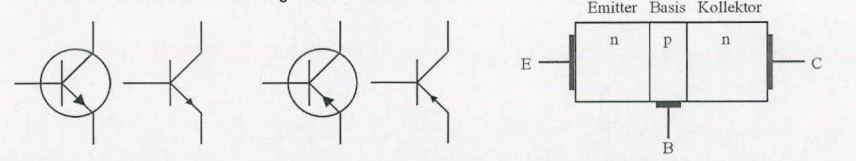
\includegraphics[scale=0.6]{Transistorschaltzeichen.jpg}	
	\caption{links: NPN, Mitte: PNP, rechts: Aufbau}
\end{figure}


\begin{figure}[h]
	\centering
	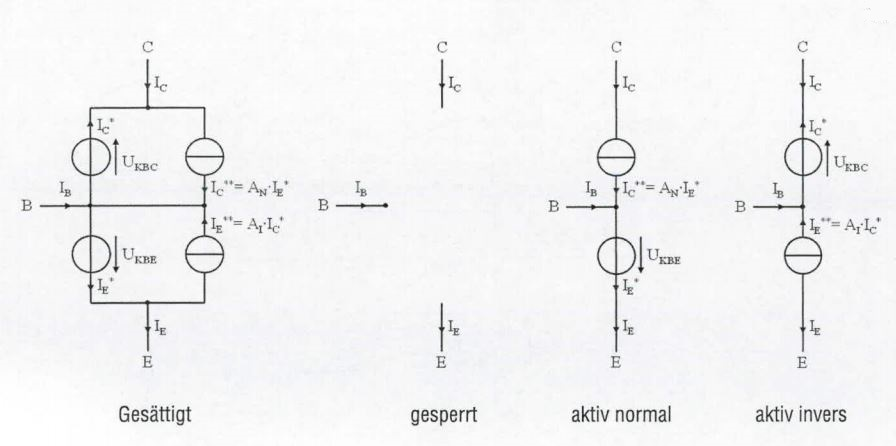
\includegraphics[scale=0.6]{Ebersmoll.jpg}	
	\caption{Ebersmoll Modell für einen Bipolartransistor}
\end{figure}


\section{Frage 7}

Werden nur Kollektor und Emitter angeschlossen (Spannung UCE > 0), entspricht dies schaltungstechnisch zwei entgegengesetzt geschalteten Dioden, von denen eine (die Basis-Kollektor-Diode) immer gesperrt ist. Es fließt nur ein kleiner Strom, der betragsgleich mit dem Sperrstrom der Basis-Kollektor-Diode ist. Die angelegte Spannung verkleinert zwar die Basis-Emitter-Sperrschicht, die Raumladungszone (RLZ) zwischen Basis und Emitter, vergrößert jedoch die Basis-Kollektor-Sperrschicht.

Durch Schließen des Basis-Emitter-Stromkreises (Spannung UBE > $U_D$ ($U_D$ entspricht der Diffusionsspannung), für Silizium $U_{BE}$ > 0,7 V) wird die Basis-Emitter-Diode leitend. Wie bei der einfachen pn-Diode werden Defektelektronen aus der Basis (p-dotiert) in den Emitter (n-dotiert) injiziert (engl. inject). Es fließt ein kleiner Basisstrom $I_{BE1}$. Im Emittergebiet klingt der Minoritätsladungsträgerüberschuss, in diesem Fall Defektelektronen, mit der Diffusionslänge ab, die Defektelektronen rekombinieren mit den Elektronen. Analog dazu werden Elektronen aus dem Emitter (lat. emittere = aussenden) in die Basis injiziert. Aufgrund der geringen Weite der Basis, die kleiner als die Diffusionslänge der Ladungsträger sein muss, rekombinieren jedoch nur wenige der Elektronen mit den Defektelektronen. Die meisten Elektronen (ca. $\unit[99]{\%}$) diffundieren durch die Basis in die Kollektor-Basis-Sperrschicht, der Basis-Kollektor-Übergang wird in Sperrrichtung betrieben. Dort driften sie wegen des großen Potentialabfalls ($U_{CB}$ > 0) in den Kollektor (lat. colligere = sammeln). In Form des Kollektorstroms IC fließen somit Elektronen vom Emitter in den Kollektor.

Die Anzahl der in das Basisgebiet injizierten Elektronen bzw. der in den Emitter injizierten Defektelektronen ändert sich mit der Flussspannung $U_{BE}$ der Basis-Emitter-Diode. Obwohl nur eine verhältnismäßig kleine Anzahl an Elektronen in der Basis rekombinieren, ist dieser Teil für die Funktion des Bipolartransistors wesentlich. Eine große Anzahl von Elektronen erhöht die Wahrscheinlichkeit, dass ein Elektron auf ein Loch trifft und rekombiniert. Die rekombinierenden Defektelektronen werden über den Basiskontakt in Form eines Teils des Basisstroms nachgeliefert. Durch Ändern des Basisstromes $I_B$ kann demzufolge der Kollektoremitterstrom IC gesteuert werden. Es wird durch den kleinen Basisstrom, verursacht durch die Defektelektronen, ein viel größerer Kollektorstrom (Elektronenstrom) gesteuert.


\href{http://de.wikipedia.org/wiki/Bipolartransistor#Ausf.C3.BChrungsbeispiele}{Quelle}


\section{Frage 8}

Es gibt drei Verschaltungsarten, die ich hier aufführe:

\begin{figure}[h]
	\centering
	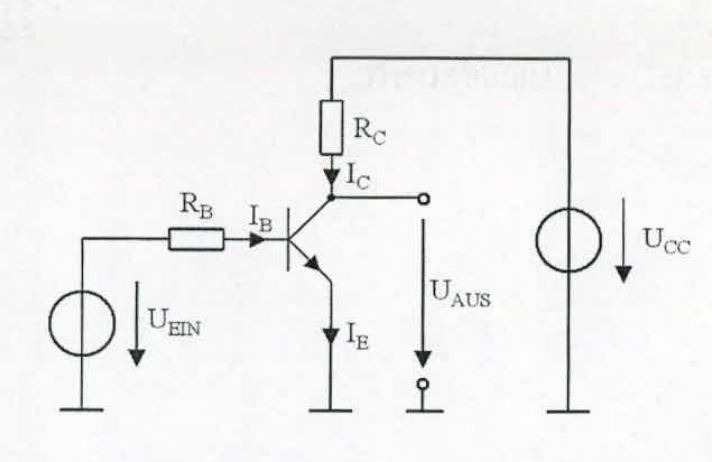
\includegraphics[scale=0.5]{Emitterschaltung.jpg}
	\caption{Die Emitterschaltung wird als Universal Verstärkerschaltung benutzt}
\end{figure}


\begin{figure}[h]
	\centering
	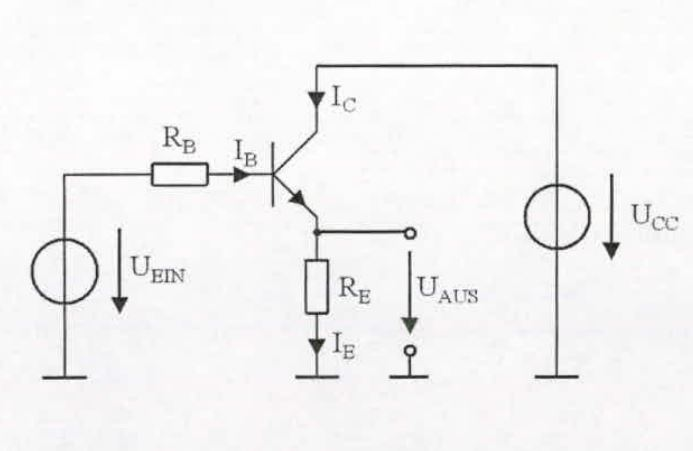
\includegraphics[scale=0.5]{Kollektorschaltung.jpg}
	\caption{Die Emitterschaltung wird als Universal Verstärkerschaltung benutzt}
\end{figure}

\begin{figure}[h]
	\centering
	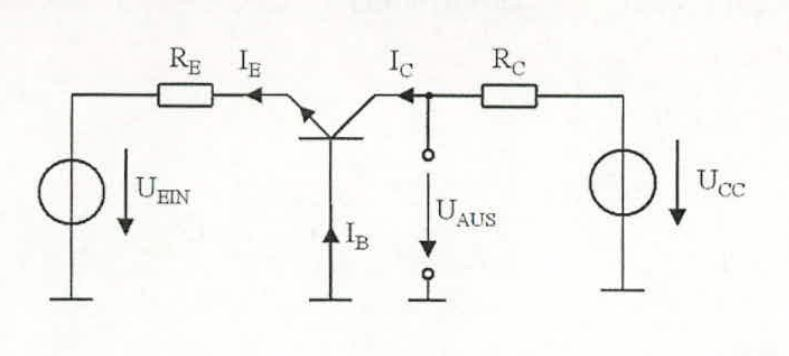
\includegraphics[scale=0.5]{Basisschaltung.jpg}
	\caption{Die Basisschaltung wird als Spannungs- und Leistungsverstärker und zum erzeugen hochfrequente Sinusschwingungen verwendet}
\end{figure}


\newpage


\section{Frage 9}


Ich weiß nicht ob das zu einem npn Transistor gehört, aber das Prinzip sollte ja bei jedem Schaltbild das selbe sein:

\begin{figure}[h]
	\centering
	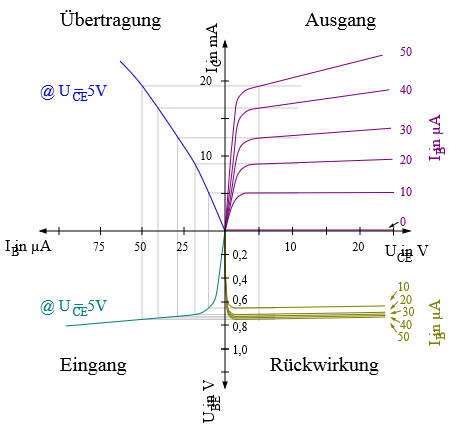
\includegraphics[scale=0.5]{Kombiniertes_Kennlinienfeld_Transistor.png}
	\caption{Vierquadrantenkennlienienfeld}
\end{figure}

\newpage


\section{Frage 10}


Die Abbildung zeigt $I_C (U_{CE})$ für verschiedene Werte von $U_{BE}$. Die Gerade, die eingezeichnet ist, nennt sich Lastgerade. Die Lastgerade besitzt die Steigung $\frac{1}{R_L}$, ihr Schnittpunkt mit der Kennlinie legt den Arbeitspunkt fest. Da der Wert von $U_{BE}$ für den aktiv normalen Betrieb nur leicht schwankt, kann man ihn mit guter Näherung zu $U_{BE} = \unit[0,7]{V}$ annehmen. 

\begin{figure}[h]
	\centering
	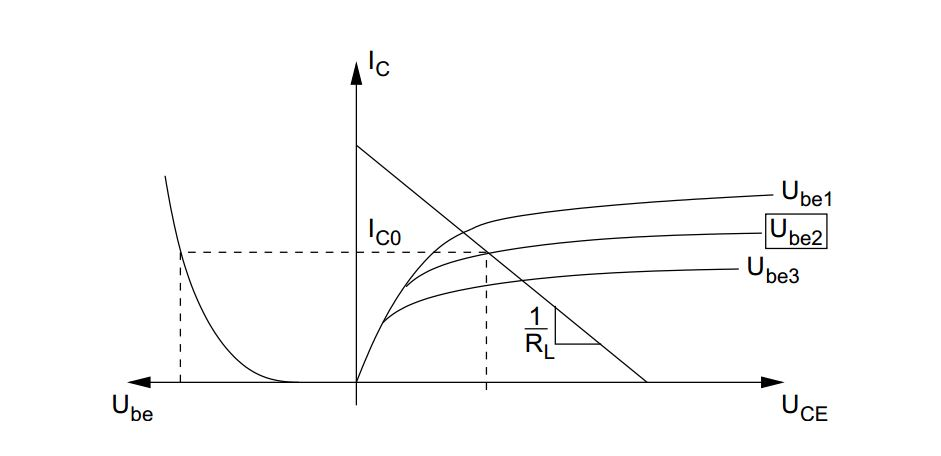
\includegraphics[scale=0.5]{Lastgerade.jpg}
	\caption{Lastgerade}
\end{figure}

Extrapoliert man den Wert für $I_C$ aud em Graphen von $I_C(U_{CE})$ in den Graphen für $I_C(U_{BE})$, so lässt sich mit dem Näherungswert für $U_{BE}$ die Spannung $U_{CE}$ aus dieser Kennline ablesen.


\href{http://www.uni-saarland.de/fileadmin/user_upload/Professoren/fr74_ProfMoeller/Praktikum/P_SS08/Transistorgrundschaltung_13_06_08.pdf}{Quelle}




\end{document}